\chapter{其他约化群的Langlands对应I：根数据与约化群}\label{L18}\lecturedate{2020/04/20}\sourcepage{148}
我们希望对约化群表述一个与Langlands对应中的相容性结论类似的命题。
\section{根数据与根系}\label{L18S1}\idx{根数据}\idx{根系}\idx{余根}\idx{Weyl群}
\begin{definition*}
\textbf{根数据}是一个四元组$\Psi=(X,\Phi,X^\vee,\Phi^\vee)$，其中$X,X^\vee$为有限秩自由阿贝尔群，并通过完美配对$\langle\ ,\ \rangle:X\times X^\vee\to\Z$互为对偶；$\Phi\subseteq X$、$\Phi^\vee\subseteq X^\vee$为有限子集，具有双射$\alpha\mapsto\alpha^\vee$\znote{根数据是约化群与其根系之间不依赖基的最小资料：$X$ 是极大环面的特征标格，$X^\vee$ 是余特征标格，$\Phi$ 与 $\Phi^\vee$ 为根与余根，由 $\alpha\mapsto\alpha^\vee$ 配对。它比根系多带了「环面部分」，因而能区分 $\SL_n$ 与 $\\operatorname{PGL}_n$ 这类根系相同而中心不同的群；对偶 $\Psi^\vee$ 交换 $X$ 与 $X^\vee$，正是 Langlands 对偶的来源。[来源：T.A. Springer, \textit{Reductive groups}, in \textit{Automorphic forms, representations and L-functions}, Proc. Symp. Pure Math. 33, Part 1, AMS 1979, pp.~3--27（本讲参考文献 [S]）。]}。还要求满足以下两条公理：
\begin{description}
\item[(RD1)] 对任意$\alpha\in\Phi$，$\langle\alpha,\alpha^\vee\rangle=2$。
\item[(RD2)] 对任意$\alpha\in\Phi$，$s_\alpha(\Phi)\subseteq\Phi$、$s_{\alpha^\vee}(\Phi^\vee)\subseteq\Phi^\vee$，其中$s_\alpha$、$s_{\alpha^\vee}$分别为$X$、$X^\vee$的自同态，定义为
\begin{equation}\tag{1.1}\label{L18eq11}s_\alpha(x)=x-\langle x,\alpha^\vee\rangle\alpha,\qquad s_{\alpha^\vee}(u)=u-\langle\alpha,u\rangle\alpha^\vee.\end{equation}
\end{description}
\end{definition*}
显然，若$\Psi=(X,\Phi,X^\vee,\Phi^\vee)$为根数据，则$\Psi^\vee=(X^\vee,\Phi^\vee,X,\Phi)$也是根数据，称为$\Psi$的\textbf{对偶}。

设$\Psi$为根数据，$Q$为$\Phi$生成的$X$的子群，令$V=Q\otimes_{\Z}\Q$。类似地定义$X^\vee$的子群$Q^\vee$及向量空间$V^\vee$。若$(Q^\vee)^\perp=\{0\}$，称$\Psi$\textbf{半单}；若$\Phi$为空，称它为\textbf{环面型}。
% [Tutor Note: 原书 p148 作 $V=Q\otimes\Q$，漏了下标 $\Z$；$Q$ 是自由阿贝尔群，其有理化应为 $V=Q\otimes_{\Z}\Q$，译文已补。]
\sourcepage{149}
假设$\Phi\ne\varnothing$。$V^\vee$可识别为$V$的对偶向量空间，仍以$\langle\ ,\ \rangle$表示配对。于是$\Phi$为$V$中的根系\znote{根系是根数据忘掉 $X,X^\vee$ 之后剩下的反射群资料：$V$ 为根张成的有理向量空间，三条公理要求每个根有唯一余根、反射 $s_\alpha$ 保持 $\Phi$、且 $\alpha^\vee$ 在 $\Phi$ 上取整值。由根数据构造时 $\Phi$ 自动张成 $V$。从根数据到根系要丢掉 $X,X^\vee$ 中与根无关的环面部分，故根系比根数据粗；Langlands 对偶必须用根数据而不能只用根系，这也是教材先讲根系、再讲根数据的原因。[来源：T.A. Springer, \textit{Reductive groups}, in \textit{Automorphic forms, representations and L-functions}, Proc. Symp. Pure Math. 33, Part 1, AMS 1979, pp.~3--27（本讲参考文献 [S]）。]}，意义如下。
\begin{definition*}
$V$中的\textbf{根系}$\Phi$满足：
\begin{description}
\item[(RS1)] $\Phi$有限、张成$V$，且$0\notin\Phi$。
\item[(RS2)] 对每个$\alpha\in\Phi$，存在$\alpha^\vee\in V^\vee$，满足$\langle\alpha,\alpha^\vee\rangle=2$，并且\eqref{L18eq11}定义的$s_\alpha$保持$\Phi$。
\item[(RS3)] 对每个$\alpha\in\Phi$，$\alpha^\vee(\Phi)\subseteq\Z$。
\end{description}
\end{definition*}
反射$s_\alpha$生成$\GL(V)$的一个子群，称为$\Phi$的\textbf{Weyl群}，记为$W(\Phi)$。由(RS1)、(RS2)，$W(\Phi)$可嵌入$\operatorname{Aut}(\Phi)$；$\Phi$为有限集，故$\operatorname{Aut}(\Phi)$及$W(\Phi)$都有限。

设$\Phi\subseteq V$为根系，令$V_{\R}:=V\otimes_{\Q}\R$。若超平面$H\subseteq V_{\R}$是某个$\alpha^\vee\in\Phi^\vee$的核，即与该余根正交，则称$H$为\textbf{奇异超平面}。\textbf{Weyl室}$C$是全部奇异超平面之并的补集的一个连通分支。每个Weyl室确定根的一个正负划分：$\alpha>0$当且仅当对所有$x\in C$，$\langle x,\alpha^\vee\rangle>0$。\idx{Weyl室}\idx{单根}
% [Tutor Note: 原书 p149 作 $V_R:=V\otimes_{\Q}\C$，并说 Weyl 室 $C$ 是 $V_\C$ 的子集；奇异超平面是实超平面，「连通分支」只在实向量空间中有意义，故应为 $V_\R:=V\otimes_{\Q}\R$，译文按 $\R$ 处理。]

对于所选的正负划分，若根$\alpha$为正根，且不能表示为两个正根之和，则称它为\textbf{单根}。单根集合$\Delta$称为$\Phi$的\textbf{基}。有以下性质。
\begin{enumerate}[label=\arabic*.]
\item $W(\Phi)$在Weyl室集合上单传递作用。
\item $s_\alpha$，$\alpha\in\Delta$，生成$W(\Phi)$；更确切地说，$(W,(s_\alpha)_{\alpha\in\Delta})$为Coxeter系统。
\item 每个根都是单根的整系数线性组合，其非零系数具有相同符号。因此$\Phi=\Phi^+\sqcup\Phi^-$。
\end{enumerate}
若根系不是两个非零子根系的直和，则称其\textbf{不可约}。若基$\Delta$不能分解为两个非空不交子集$\Delta'\sqcup\Delta''$，使$(\Delta'+\Delta'')\cap\Phi=\varnothing$，则称$\Delta$\textbf{连通}。有：$\Phi$不可约当且仅当$\Delta$连通。

若对每个$\alpha\in\Phi$，$\Phi$中与$\alpha$成比例的根只有$\pm\alpha$，则称$\Phi$\textbf{约化}。
\sourcepage{150}
\textbf{带基根数据}是六元组$\Psi_0=(X,\Phi,\Delta,X^\vee,\Phi^\vee,\Delta^\vee)$，其中$(X,\Phi,X^\vee,\Phi^\vee)$为根数据，$\Phi$约化，$\Delta$为$\Phi$的一组基。带基根系由Dynkin图分类，其中不可约根系对应连通Dynkin图。
\section{约化群}\label{L18S2}\idx{幺幂群}\idx{根基}\idx{Borel子群}
设$k$为域，除非另有说明，假设$k$代数闭。本节的约化群默认连通。\textbf{线性代数$k$群}$G$是具有群结构的仿射簇，且全部群运算为正则映射。特别地，乘法和求逆由代数簇态射$\mu:G\times G\to G$、$\rho:G\to G$给出，等价地由$k$-代数同态
\[\mu^\natural:k[G]\to k[G]\otimes_k k[G],\qquad\rho^\natural:k[G]\to k[G]\]
给出。每个$k$群$G$都有相应Lie代数$\g$，$G$在$\g$上有自然的伴随作用。

连通$k$群$G$\textbf{可解}，当且仅当存在群嵌入$G\hookrightarrow\GL_n(k)$使其像包含于上三角矩阵群。
% [Tutor Note: 原书 p150 作 $G\hookrightarrow\GL(k)$，漏了下标 $n$；按上下文应为 $G\hookrightarrow\GL_n(k)$，译文已补。]$G$\textbf{幺幂}，当且仅当可将其嵌入对角元全为$1$的上三角矩阵群。$G$的最大连通正规可解子群称为\textbf{根基}，记为$R(G)$。事实上，
\[R(G)=\Bigl(\bigcap_{B\subseteq G\text{为Borel子群}}B\Bigr)^0.\]
$G$的最大连通正规幺幂子群称为\textbf{幺幂根基}，记为$R_u(G)$。
\originalnumber{1}
\begin{definition}\label{L18S2O1}
\begin{enumerate}[label=(\arabic*)]
\item 若$R(G)$为环面，等价地，若$R_u(G)$平凡，则称$G$\textbf{约化}\znote{约化即「根基是环面」或等价地「幺幂根基平凡」，直观上是从 $G$ 中剥掉幺幂部分后剩下的群；$\GL_n$、$\SL_n$、$\SO_n$、$\\operatorname{Sp}_{2n}$ 都是约化群。约化比半单多一个中心环面因子，特征零时约化群的 Lie 代数约化（伴随表示完全可约）。易错点：约化（reductive）不等于线性约化（linearly reductive，指表示完全可约）；特征 $p>0$ 时 $\GL_p$ 约化却非线性约化。[来源：T.A. Springer, \textit{Reductive groups}, in \textit{Automorphic forms, representations and L-functions}, Proc. Symp. Pure Math. 33, Part 1, AMS 1979, pp.~3--27（本讲参考文献 [S]）。]}。
\item 若连通$k$群$G$的$R(G)$平凡，则称$G$\textbf{半单}。在特征零时，这等价于其Lie代数$\g$半单。
\end{enumerate}
\end{definition}
在代数闭的特征零域上，半单Lie代数与约化根系的同构类一一对应。设$G$为连通约化$k$群。对任意子环面$S\subseteq G$，将$S$在$\g$上的伴随表示对角化，出现的非平凡特征标集合记为$\Phi(G,S)$。
\sourcepage{151}

\originalnumber{2}
\begin{example}\label{L18S2O2}
令$G=\SL_2(\C)$，$S=\{\operatorname{diag}(a,b)\mid ab=1\}$。选取$\g$的基
\[e=\begin{pmatrix}0&1\\0&0\end{pmatrix},\quad f=\begin{pmatrix}0&0\\1&0\end{pmatrix},\quad h=\begin{pmatrix}1&0\\0&-1\end{pmatrix}.\]
在此基下，伴随表示为
\[\rho:S\longrightarrow\GL(\g)\cong\GL_3(\C),\qquad\operatorname{diag}(a,b)\longmapsto\operatorname{diag}(ab^{-1},a^{-1}b,1).\]
% [Tutor Note: 原书 p151 在此基 $(e,f,h)$ 下把矩阵写作 $\operatorname{diag}(a^{-1}b,ab^{-1},1)$；但 $e=E_{12}$ 的重量为 $ab^{-1}$、$f=E_{21}$ 的重量为 $a^{-1}b$（见同一页 $\chi_\pm=(a^{-1}b)^{\pm1}$ 的指标约定），故按所列基序应为 $\operatorname{diag}(ab^{-1},a^{-1}b,1)$，译文按后者处理。]
因此$(e,f,h)$将$S$的伴随表示对角化。此外，$\Phi(G,S)=\{\chi_+,\chi_-\}$，其中$\chi_\pm(\operatorname{diag}(a,b))=(ab^{-1})^{\pm1}$。
\end{example}
固定$G$的极大环面$T$\znote{极大环面是 $G$ 中维数最大的环面子群。代数闭域上所有极大环面彼此共轭，且共轭可由 Weyl 群实现，故根数据 $\Psi(G,T)$ 不依赖 $T$ 的选取。$\GL_n$ 的对角环面、$\SO_n$ 的旋转环面都是极大环面。分裂约化群正是「存在定义于 $k$ 且在 $k$ 上分裂的极大环面」的群，因此其根数据可直接用 $X^*(T)$ 描述。[来源：nLab "maximal torus"，\url{https://ncatlab.org/nlab/show/maximal+torus}（Last revised 2026-04-28；2026-11-14 访问）。]}。对应于$(G,T)$的根数据为$\Psi(G,T)=(X,\Phi,X^\vee,\Phi^\vee)$。这里$X=X^*(T)$为$T$的代数特征标群，$X^\vee=X_*(T)$为$T$的一参数乘法子群，即余特征标群。配对定义为
\[\langle x,u\rangle\in\Z,\qquad x(u(t))=t^{\langle x,u\rangle},\quad u:\mathbb G_m\to T,\ x:T\to\mathbb G_m.\]
根系$\Phi$为$\Phi(G,T)$。接下来描述$\Phi^\vee$。对$\alpha\in\Phi(G,T)$，令$T_\alpha$为$\ker\alpha$的单位连通分支。$T_\alpha$在$G$中的中心化子$Z_\alpha$为连通约化群，具有极大环面$T$；其导出群$G_\alpha:=[Z_\alpha,Z_\alpha]$为秩一半单群。实际上，$T$在$\g$上的伴随作用给出分解
\begin{equation}\tag{2.1}\label{L18eq21}\g=\mathfrak t\oplus\bigoplus_{\beta\in\Phi}\g_\beta,\end{equation}
其中$\mathfrak t=\operatorname{Lie}(T)$，且$\dim_k\g_\beta=1$。$Z_\alpha$的Lie代数为$\mathfrak t\oplus\g_\alpha\oplus\g_{-\alpha}$，$T_\alpha$以有限核映到$Z_\alpha/G_\alpha$。
% [Tutor Note: 原书 p151 作「$T_\alpha$ maps identically to its image in $Z_\alpha/G_\alpha$」；实际 $\ker(T_\alpha\to Z_\alpha/G_\alpha)=T_\alpha\cap G_\alpha\subset\mu_2$ 有限，同态并非同构，译文按「以有限核」处理。]$G_\alpha$包含一维环面；在特征零时，$\operatorname{Lie}(G_\alpha)\cong\mathfrak{sl}_2(k)=kh\oplus ke\oplus kf$，其中$h,e,f$如\eref{例题}{L18S2O2}。
\sourcepage{152}
存在唯一的余根同态$\alpha^\vee:\mathbb G_m\to G_\alpha$，其像位于$T$中，并满足$\langle\alpha,\alpha^\vee\rangle=2$。乘法映射$\operatorname{Im}(\alpha^\vee)\times T_\alpha\to T$为同源。在上述特征零的Lie代数识别下，$\alpha^\vee$的像的Lie代数为$kh$。
% [Tutor Note: 原书 p152 作 $T=(\operatorname{Im}\alpha^\vee)\times T_\alpha$ 且 $\langle\alpha,\alpha^\vee\rangle$ 后缺 $=2$；乘法映射 $\operatorname{Im}(\alpha^\vee)\times T_\alpha\to T$ 只在交为 $\operatorname{Im}\alpha^\vee\cap T_\alpha$（有限）的意义下是同源，译文按此处理。]
\originalnumber{3}
\begin{example}\label{L18S2O3}
令$G=\SL_2(\C)$，$T=\{\operatorname{diag}(a,b)\mid ab=1\}$。已经看到$\Phi(G,T)=\{\chi_+,\chi_-\}$，$\chi_\pm(\operatorname{diag}(a,b))=(ab^{-1})^{\pm1}$。所有特征标可写为$\chi_{(n,m)}(\operatorname{diag}(a,b))=a^nb^m$；由于$ab=1$，有
\[X^*(T)\cong\Z^2/\Z(1,1)\cong\Z.\]
% [Tutor Note: 原书 p152 例 2.3 作 $X\cong\Z^2$，漏了关系 $ab=1$；正确为 $X^*(T)\cong\Z^2/\Z(1,1)\cong\Z$，译文已补。]
$T_{\chi_\pm}$平凡，相应余根为
\[\chi_\pm^\vee(t)=\operatorname{diag}(t^{\pm1},t^{\mp1}).\]
\end{example}
有以下定理。
\originalnumber{4}
\begin{theorem}\label{L18S2O4}
设$k$代数闭。对任意根系约化的根数据$\Psi$，都存在连通约化群$G$及其极大环面$T\subseteq G$，满足$\Psi=\Psi(G,T)$。$(G,T)$在相差同构的意义下唯一。
\end{theorem}
我们已经说明如何从约化群得到根数据。反过来，给定根数据$\Psi=(X,\Phi,X^\vee,\Phi^\vee)$，希望构造约化群$G_\Psi$。以下给出特征零下的一种构造。先选取单根集$\Delta$，考虑范畴$C(\Psi)$，其对象和态射如下。
\begin{enumerate}[label=(\arabic*)]
\item 对象为有限维$k$向量空间族$(V_\mu)_{\mu\in X}$，以及对$\mu\in X$、$\alpha\in\Delta$给出的算子$e_\alpha:V_\mu\to V_{\mu+\alpha}$、$f_\alpha:V_\mu\to V_{\mu-\alpha}$，满足：
\begin{enumerate}[label=(\alph*)]
\item $\{\mu\mid V_\mu\ne0\}$为有限集；
\item $[e_\alpha,f_\beta]|_{V_\mu}=\delta_{\alpha\beta}\langle\mu,\alpha^\vee\rangle\mathrm{Id}_{V_\mu}$，其中
\[[e_\alpha,f_\beta]=e_\alpha f_\beta-f_\beta e_\alpha:V_\mu\to V_{\mu+\alpha-\beta}.\]
% [Tutor Note: 原书 p152 (1)(b) 把 $[e_\alpha,f_\beta]$ 的限制下标误作 $V_\alpha$，应为 $V_\mu$（与同一行的 $\langle\mu,\alpha^\vee\rangle$ 一致）；译文已改用 $V_\mu$。]

\end{enumerate}
\sourcepage{153}
\item 态射为线性映射族$(\varrho_\mu)_{\mu\in X}$，对任意$\mu\in X$、$\alpha\in\Delta$，与$e_\alpha,f_\alpha$的作用相容，使下图交换：
\begin{figure}[H]\centering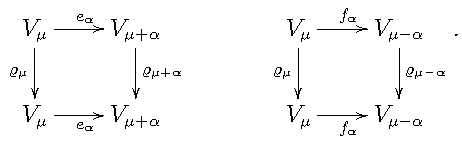
\includegraphics[width=0.3727\paperwidth]{images/L18-p153-morphisms.pdf}\end{figure}
\end{enumerate}
$C(\Psi)$自然具有刚性张量范畴结构。遗忘函子$\mathfrak F:C(\Psi)\to\operatorname{Vect}_k$将$(V_\mu)$送到$\bigoplus_\mu V_\mu$，是张量函子。定义$k$群$G_\Psi:=\operatorname{Aut}(\mathfrak F,\otimes)$，则它恰为根数据$\Psi$所对应的约化群。此外，由Tannaka形式理论，有张量范畴等价$C(\Psi)\simeq\operatorname{Rep}(G_\Psi)$。

回忆，$k$群$G$的\textbf{Borel子群}是极大连通可解子群。固定极大环面后，选取包含它的Borel子群，等价于选取一组正根。

现在设$k$为任意域，$k^s$、$\overline k$分别为可分闭包和代数闭包。若光滑连通$k$群$G$在代数闭包上的基变换$G_{\overline k}$按\eref{定义}{L18S2O1}为约化群，则称$G$约化。若连通约化$k$群$G$含有一个定义于$k$的Borel子群，则称它\textbf{拟分裂}。若$G$具有一个定义于$k$且在$k$上分裂的极大环面，则称它\textbf{分裂}。分裂群一定拟分裂。拟分裂性一般是相当强的限制，不过有：\idx{拟分裂群}\idx{分裂群}
% [Tutor Note: 原书 p153 定义约化 $k$ 群时用 $G\times_k k^s$（可分闭包），译文统一改用 $\overline k$；在本讲义涉及的有限域与曲线情形 $k^s=\overline k$，读者对照其他文献时注意这一差别。]
\begin{itemize}
\item 若$k$为有限域，则任意连通约化$k$群均拟分裂，这是Lang定理的结果。
\item 若$k$为非阿基米德局部域，则对每个连通约化$k$群$G$，存在非分歧扩张$L/k$，使$G$在$L$上拟分裂。
\item 若$k$为整体域，则对几乎所有素位$v$，$G\times_k k_v$拟分裂。
\end{itemize}
\sourcepage{154}
设$G$为连通约化$k$群，$S$为极大$k$-分裂环面，即$G$的$k$子环面，且$S$在$k$上分裂并对这一性质极大。$\dim S$称为$G$的\textbf{$k$-秩}。一般而言，$S$未必是$G$的极大环面。$\Phi(G,S)$称为$G$的\textbf{相对根系}\znote{绝对根系在代数闭包上取值，相对根系 ${}_k\Phi$ 只记录在 $k$ 上可见的根：取极大 $k$-分裂环面 $S$，把 $\operatorname{Lie}G$ 对 $S$ 对角化即得。$G$ 分裂时两者一致；非分裂时 ${}_k\Phi$ 可能不约化、根空间维数也可能大于 $1$。$k$-秩 $\dim S$ 衡量 $G$ 在 $k$ 上能分裂出多少环面，它正是 Satake 参数中与 $L$ 群相关的量。[来源：T.A. Springer, \textit{Reductive groups}, in \textit{Automorphic forms, representations and L-functions}, Proc. Symp. Pure Math. 33, Part 1, AMS 1979, pp.~3--27（本讲参考文献 [S]）。]}，记为${}_k\Phi$。相应的Lie代数分解为
\begin{equation}\tag{2.2}\label{L18eq22}\g=\g_0\oplus\bigoplus_{\alpha\in{}_k\Phi}\g_\alpha,\end{equation}
其中$\g_0$为中心化子$Z(S)$的Lie代数。若$G$在$k$上分裂，则$S$为$G$的极大环面，${}_k\Phi$与绝对根系$\Phi(G_{\overline k},S_{\overline k})$一致。一般而言，相对根系未必约化，根空间$\g_\alpha$也未必为一维。\idx{相对根系}
% [Tutor Note: 原书 p154 在此写绝对根系为 $\Phi(G(k),S(k))$；绝对根系应在代数闭包上取，即 $\Phi(G_{\overline k},S_{\overline k})$，译文已按此处理。]
\originalnumber{5}
\begin{definition}\label{L18S2O5}\idx{Langlands对偶群}
设$G$为根数据$\Psi=(X,\Phi,X^\vee,\Phi^\vee)$对应的分裂约化群。对偶根数据$\Psi^\vee$给出另一个分裂约化群$G^\vee$，称为$G$的\textbf{Langlands对偶群}\znote{对偶根数据 $\Psi^\vee$ 把特征标格与余特征标格互换，对应群 $G^\vee$（常记 $G^L$）。例：$\SL_n$ 与 $\\operatorname{PGL}_n$ 互为对偶，$\\operatorname{Sp}_{2n}$ 与 $\SO_{2n+1}$ 互为对偶，$\GL_n$ 自对偶。直观上 $G$ 与 $G^\vee$ 根系相同而中心、余中心互换，故 $G^\vee$ 的极大环面是 $G$ 极大环面的对偶环面。完整的 $L$ 群还带 Galois 部分，本讲只处理分裂情形。[来源：T.A. Springer, \emph{Reductive groups}, in \emph{Automorphic forms, representations and $L$-functions}, Proc. Symp. Pure Math. 33, Part 1, pp. 3--27, AMS, 1979（本讲参考文献 [S]）。]}，有时记为$G^L$。
\end{definition}
\originalnumber{6}
\begin{example}\label{L18S2O6}
\begin{center}\begin{tabular}{c|c}$G$&$G^L$\\\hline$\GL_n$&$\GL_n$\\$\SL_n$&$\operatorname{PGL}_n$\\$\operatorname{Sp}_{2n}$&$\SO_{2n+1}$\end{tabular}\end{center}
\end{example}
$k$群$G$的\textbf{有理表示}，由$k$向量空间$V$及$k$群同态$\rho:G\to\GL(V)$组成。关于分裂约化群的表示论，有下面的重要定理。若权$\lambda\in X=X^*(T)$满足$\langle\lambda,\alpha^\vee\rangle\ge0$，$\alpha\in\Delta$，则称$\lambda$为\textbf{支配权}。\idx{支配权}
% [Tutor Note: 原书 p154 作「A weight $\lambda\in X^\vee$ is dominant if $\langle\alpha,\lambda\rangle\ge0$」；支配权是 $X=X^*(T)$ 中的元素，条件应为 $\langle\lambda,\alpha^\vee\rangle\ge0$，译文已改正。]
\originalnumber{7}
\begin{theorem}\label{L18S2O7}
分裂约化群$G$的不可约有理表示的同构类，与$G$的支配权一一对应。
\end{theorem}
还要提及两个与约化性相关的定义。
\originalnumber{8}
\begin{definition}\label{L18S2O8}
\begin{enumerate}[label=(\arabic*)]
\item 若线性代数群$G$满足下列两个等价条件之一，则称它\textbf{线性约化}：
\begin{enumerate}[label=(\alph*)]
\item 每个有限维有理线性表示均完全可约，即是不可约表示的直和；
\sourcepage{155}
\item 对每个有理表示$\rho:G\to\GL(V)$及任意非零$\rho(G)$-不变向量$v\in V$，存在$\rho(G)$-不变线性函数$f$，满足$f(v)\ne0$。
% [Tutor Note: 原书 p155 (1)(b) 作 $f(W)\ne0$；此处 $W$ 未定义，应为 $f(v)\ne0$，译文已按 $f(v)\ne0$ 处理。]
\end{enumerate}
\item 若对每个有理表示$\rho:G\to\GL(V)$及任意非零不变向量$v\in V$，存在正次数的$\rho(G)$-不变齐次多项式函数$f$，使$f(v)\ne0$，则称$G$\textbf{几何约化}，亦称\textbf{半约化}。
% [Tutor Note: 原书 p155 (2) 作「non-constant polynomial function」；结合不变性可取其齐次分量，故与「正次数齐次多项式」等价，译文按后者表述。]
\end{enumerate}
\end{definition}
任意线性约化群都是约化群；线性代数群约化当且仅当几何约化。最后，若$\operatorname{char}(k)=0$，则$G$约化当且仅当$G$线性约化。
\section{环上的约化群}\label{L18S3}\idx{群概形}\idx{良约化}
可以将域$k$换成交换环$R$，得到\textbf{$R$上的仿射群概形}，简称\textbf{$R$群}。以$G(R)$表示$G$的$R$-点群，以$R[G]$表示$G$的坐标代数。若$R'$为$R$-代数，则基变换给出$R'$群$G\times_R R'$，其坐标代数为$R'[G]$。设$\mathfrak m$为$R$的极大理想，令$k(\mathfrak m)=R/\mathfrak m$。
\originalnumber{1}
\begin{definition}\label{L18S3O1}
设$G$为平坦且有限表示的$R$群。若$G\times_R k(\mathfrak m)$为光滑$k(\mathfrak m)$群，则称$G$在$\mathfrak m$处具有\textbf{良约化}。若$G$在所有极大理想处均具有良约化，则称$G$为\textbf{光滑}$R$群。
% [Tutor Note: 原书 p155 定义 3.1 作「$G\times_R k(\mathfrak m)$ is a $k(\mathfrak m)$-group」，漏了「光滑」；任何基变换都是 $k(\mathfrak m)$-群，故该条件只有读作「光滑 $k(\mathfrak m)$-群」才有意义，译文已补。]
\end{definition}
设$G$为域$k$上的$k$群，$R\subseteq k$为子环。若存在光滑$R$群$G_0$，满足$G\cong G_0\times_R k$，则称$G$\textbf{可定义于}$R$。
\originalnumber{2}
\begin{note}[L18S3O2]
由Chevalley定理，复连通半单群可定义于$\Z$。
\end{note}
还可以令$R=\A$为整体域$k$的阿代尔环。$G(\A)$为$\A$-点群，称为$G$的\textbf{阿代尔群}。由\sref{L4S2}，$G(\A)$局部紧，并包含对角嵌入的离散子群$G(k)$。
\sourcepage{156}
\needspace{5\baselineskip}\section{第18讲参考文献}\label{L18S4}
\begin{references}
\refitem{L18bibS}{S} T.A. Springer, \emph{Reductive groups}, in \emph{Automorphic forms, representations and L-functions}, Proc. Symp. Pure Math. 33, Part 1, pp. 3--27, AMS, 1979.
\end{references}
